\newpage\EMPHASIZE{80. Inheritance}

\textsc{Objectives}

\begin{tightlist}
\item
  Understand inheritance
\item
  Understand how to call the constructor of the superclass
\item
  Understand how the destructor of the superclass is called
\item
  Understand how a method can hide a method of the same signature in the
  superclass
\item
  Understand how a member variable can hide a member variable in the
  superclass
\item
  Understand how to call a hidden method in the superclass
\item
  Understand how names are found by the compiler in an inheritance
  hierarchy
\item
  Understand the difference between composition and inheritance
\item
  Understand how to choose between composition and inheritance
\item
  Understand multiple inheritance
\item
  Understand protected members
\item
  Understand public, protected, and private inheritance
\end{tightlist}

\newpage\EMPHASIZE{The problem}

Instead of working with classes (and their objects) alone, we can work
with a hierarchy of classes. Why do we want to do this? To improve
``re-use''.

For instance: Suppose you have an \texttt{Employee} class and you want to
create a \texttt{Manager} class. A manager \EMPHASIZE{is an} employee -\/-
everything in the \texttt{Employee} class should be in the \texttt{Manager}
class. For instance an \texttt{Employee} might have a last name,
\texttt{Manager} should have a last name too.

You basically want the \texttt{Manager} class to have all the member
variables and methods of the \texttt{Employee} class. Of course you can
copy-and-paste the code from the \texttt{Employee }class into the
\texttt{Manager} class:
\begin{console}
class Employee
{
public:
        ...
        std::string get_firstname();
        void set_firstname(const std::string &);
private:
        std::string firstname;
        ...
};

class Manager
{
public:
        ...
        std::string get_firstname();
        void set_firstname(const std::string &);
        // other stuff not from Employee class
        ...
private:
        std::string firstname;
        // other stuff not from Employee class
        ...
}; 
\end{console}

Of course you would expect the \texttt{Manager} class to contain more
things than the \texttt{Employee} class. For instance in the company where
the above software is written, a manager might have a secretary while
non-managers do not.

We don't like to duplicate code. If you need to modify the code from the
\texttt{Employee} class, then you also need to modify the same code in the
\texttt{Manager} class. And if code in the \texttt{Employee} class is used
in 10 other classes, the maintenance work on code would be horrific.

What should we do?

\newpage\EMPHASIZE{Inheritance}

The solution is to use \EMPHASIZE{inheritance}!!!

The general idea is very simple: Basically C++ allows you to define a
class so that it will have all the ``features'' of another.

That's all. BUT ... there is \EMPHASIZE{a lot} of details beyond the
general idea of inheritance. So \EMPHASIZE{pay attention}.

Here is the basic syntax to get a class to inherit ``features'' from
another class:
\begin{console}[commandchars=\~\@\$]
class Employee
{ ... };
class Manager: ~EMPHASIZE@public Employee$
{ ... }; 
\end{console}

This is called \EMPHASIZE{public inheritance}, i.e., the \texttt{Manager}
class \EMPHASIZE{inherits} everything (i.e. member variables and methods)
of the \texttt{Employee} class in the sense that the \texttt{Manager} class
will have all the features (member variables and methods) from the
\texttt{Employee} class.

Here is some basic terminology that you must know:

\begin{itemize}
\item
  \texttt{Employee} is the \EMPHASIZE{parent class} or the
  \EMPHASIZE{superclass} and \texttt{Manager} is the \EMPHASIZE{child class} or
  the \EMPHASIZE{subclass}.
\item
  \texttt{Manager} is \EMPHASIZE{derived} from \texttt{Employee} or
  \texttt{Manager} is a \EMPHASIZE{derived subclass} of \texttt{Employee}.
\end{itemize}

I'm going to use the following very simple example to illustrate
important principles when working with inheritance.

\begin{itemize}
\item
  The parent class \texttt{P} has the integer member \verb!x_! together
  with \verb!get_x! and \verb!set_x! methods.
\item
  The child class \texttt{C} has an integer member \verb!y_! together
  with \verb!get_y! and \verb!set_y! methods.
\end{itemize}

I don' t have to tell you ... run it.
%sidenote tikzbox here
\begin{console}
#include <iostream>

class P
{
public:
        P() : x_(1) {}
        int get_x() const { return x_; }
        void set_x(int x) { x_ = x; }
private:
        int x_;
};

class C : public P
{
public:
        C() : y_(2) {}
        int get_y() const { return y_; }
        void set_y(int y) { y_ = y; }
private:
        int y_;
};

int main()
{   
    C c;
    std::cout << "c.x_ =" << c.get_x() << ", "
              << "c.y_ =" << c.get_y() << '\n';
return 0;

} 
\end{console}

Notice that the \texttt{c} object of class \texttt{C} inherits \verb!x_!,
\verb!get_x!, and \verb!set_x! from \texttt{P}. That's why you can
execute \verb!c.get_x()! even though class \texttt{C} does not have a
\verb!get_x()! method.

Make sure you keep the above code handy since I'll be using this again
and again in this set of notes. I'm going to call the above program our
``Basic Example''.

\begin{ex} Get rid of the inheritance clause in our Basic Example:
\begin{console}[commandchars=\~\@\!]
...
class P
{
      ...
};
class C : ~EMPHASIZE@~redtext@~sout@public P!!!
{     
      ...
};
\end{console}
and compile your code again. See the error? Now you cannot execute \verb!c.get_x()!. READ the error message carefully. So we see that object \verb!c! does seem to have the \verb!get_x! method! (Put the ``\verb!: public P!'' back into the code after you're done with this exercise.)
\end{ex}

\begin{ex} Does \verb!c! have the \verb!set_x}! method? How
would you check that?
\end{ex}

\begin{ex} Does \verb!c! have the \verb!x_! member variable?
How would you check that? (Make \verb!x_! public and print \verb!c.x_! in \verb!main()!.)
\end{ex}

So \verb!C! seems to have a ``copy'' of \verb!P!'s
declaration in it. Is that so? There are lots of other questions:

\begin{itemize}
\item
  What about the private section of \verb!P!? Can \verb!C! define
  methods to access the private members of \verb!P!? If inheritance is a
  message to the compiler to ``copy-and-paste'' code from \verb!P! to
  \verb!C!, then surely methods in \verb!C! can access the private
  members of \verb!P!. Is that so?
\item
  Also, what if \verb!C! uses some features of \verb!P! but not all --
  and in fact some features need to be modified. What can we do?
\item
  What about constructor? Clearly \verb!P::P()! constructor was called
  since in the above experiment \verb!x_! is clearly 1. Can we call a
  parent constructor explicitly so that we can initialize the
  \verb!x_!?
\item
  What about object destruction?
\item
  Etc., etc., etc.!!!
\end{itemize}

\begin{ex}
The inheritance stack can be as tall as you like. Create a class \verb!G! (``grandparent'') with integer member \verb!z_! and with \verb!get_z! and \verb!set_z! method. Let the default constructor of \verb!G! initialize \verb!z_! to \verb!42!. Let class \verb!P! inherit class \verb!G!. In \verb!main()!, print the value of \verb!c.z_!.
\end{ex}

\newpage\EMPHASIZE{Inheritance is not copy-and-paste of code!}

It's really important to understand that inheritance is not a copy-and-paste of code from the parent class to the child class. Inheritance is not like your \lq\lq \verb!#include!'' business.

Here's how you should visualize objects created from a class that's a child class. Look at our Basic Example code again. We have a \verb!c! object declared with class \verb!C! which inherits class \verb!P!. The object \verb!c! has member \verb!y_!, \verb!get_y!, and \verb!set_y! since the type of \verb!c! is class \verb!C!. From the experiments in the previous section, we see that \verb!c! also has \verb!gx_!, \verb!get_x!, and \verb!set_x! from its parent \verb!P!.

Here's a picture to keep in mind. First here's a diagram of our classes:
\begin{python}
from latextool_basic import *
p = Plot()
pbox = Rect(0, 0, 2, 2, label='P', linewidth=0.1)
cbox = Rect(0,-4,2,-2, label='C', linewidth=0.1)
c2p = Line(points=[(cbox.center, cbox.top),(pbox.center, pbox.bottom)], linewidth=0.1, endstyle='>')
p += pbox
p += cbox
p += c2p
\end{python}
Each box represents the class. The arrow describes the inheritance
relationship between the two classes. (This is the so-called class
diagram from UML. I'm simplifying it a little -- see previous notes for
details on what to draw inside the boxes.) We created an object \verb!c!
from class \verb!C!. So informally I'll draw it this way:
%% \begin{python}
%% from latextool_basic import *
%% p = Plot()
%% p += Rect(0, 0, 1, 1, name='a')
%% p += Rect(2, 0, 3, 1, name='b')
%% p += ellipse(center=(5,2), width=2, height=1, name='c')
%% p += fit(name='X', names=['a', 'b', 'c'], linecolor='red')
%% print(p)
%% \end{python}
We also know that through inheritance, \verb!c! also has \verb!x_!,
\verb!get_x!, and \verb!set_x!. So where's \verb!c.x_!,
\verb!c.get_x!, and \verb!c.set_x!?

Now if you think of \verb!c.x_!, \verb!c.get_x!, and \verb!c.set_x!
in the same bag of things like this:
%% \begin{python}
%% from latextool_basic import *
%% p = Plot()
%% p += Rect(0, 0, 1, 1, name='a')
%% p += Rect(2, 0, 3, 1, name='b')
%% p += ellipse(center=(5,2), width=2, height=1, name='c')
%% p += fit(name='X', names=['a', 'b', 'c'], linecolor='red')
%% print(p)
%% \end{python}
then you would be surprised by the following experiment: Add an integer
member variable to class \verb!C!:

\begin{console}[commandchars=\~\@\$]
#include <iostream>

class P
{
public:
        P() : x_(1) {}
        int get_x() const { return x_; }
        void set_x(int x) { x_ = x; }
private:
        int x_;
};

class C : public P
{
public:
        C() : y_(2) {}
        int get_y() const { return y_; }
        void set_y(int y) { y_ = y; }
private:
        ~EMPHASIZE@~redtext@int x_;$$
        int y_;
};

int main()
{   
    C c;
    std::cout << "c.x_ =" << c.get_x() << ", "
              << "c.y_ =" << c.get_y() << '\n';
    return 0;
}
\end{console}

The program does compile. But this means that \verb!c_! now has two
\verb!x_!'s!!!
%% \begin{python}
%% from latextool_basic import *
%% p = Plot()
%% p += Rect(0,0,1,1,name='a')
%% p += Rect(2,0,3,1,name='b')
%% p += ellipse(center=(5,2), width=2, height=1, name='c')
%% p += fit(name='X', names=['a', 'b', 'c'], linecolor='red')
%% print(p)
%% \end{python}
When you call upon \verb!c.x_! which one is it??? Why does the compiler
allow this?

\begin{ex} Can you think of an experiment that can tell you
which \verb!x_! is used if you access \verb!c.x_! in \verb!main()!?
\end{ex}
You really want to think of the members (member variables as well as
methods) as being organized into two different scopes:
%% \begin{python}
%% from latextool_basic import *
%% p = Plot()
%% p += Rect(0,0,1,1,name='a')
%% p += Rect(2,0,3,1,name='b')
%% p += ellipse(center=(5,2), width=2, height=1, name='c')
%% p += fit(name='X', names=['a', 'b', 'c'], linecolor='red')
%% print(p)
%% \end{python}
The members of \verb!c! that are due to inheritance is at the top while
the members declared in class \verb!C! are at the bottom. In particular
the \verb!x_! declared in class \verb!C! is at the bottom.

The name \verb!c.x_! refers to the \verb!x_! at the bottom, i.e., the
\verb!x_! due to the class \verb!C!. Of course now you have a problem:
what if in \verb!main()!, you want to access the \verb!x_! at the
top???

In fact to be very precise, each member of \verb!c! belongs to one of
the two bags (bottom and top) and you can think of the two bags as
scopes. You can in fact specify the scopes when you access a member of
\verb!c!. First of all the scopes have names: they are \verb!C! and
\verb!P!, i.e., the names of the classes:
%% \begin{python}
%% from latextool_basic import *
%% p = Plot()
%% p += Rect(0,0,1,1,name='a')
%% p += Rect(2,0,3,1,name='b')
%% p += ellipse(center=(5,2), width=2, height=1, name='c')
%% p += fit(name='X', names=['a', 'b', 'c'], linecolor='red')
%% print(p)
%% \end{python}
You can actually address a particular member by prepending it with
\verb!C::! or \verb!P::! if you want to be specific. Try the following:
\begin{console}[commandchars=\~\@\$]
#include < iostream>

class P
{
public:
        P() : x_(1) {}
        int get_x() const { return x_; }
        void set_x(int x) { x_ = x; }
private:
        int x_;
};

class C : public P
{
public:
        C() : y_(2) {}
        int get_y() const { return y_; }
        void set_y(int y) { y_ = y; }
private:
        int x_;
        int y_;
};

int main()
{   
    C c;        
    std::cout << "c.x_ =" << c.get_x() << ", "
              << "c.y_ =" << c.get_y() << '\n';
    std::cout << "c.x_ =" << c.~EMPHASIZE@~redtext@P::$$get_x() << ", "
              << "c.y_ =" << c.~EMPHASIZE@~redtext@C::$$get_y() << '\n';
return 0;

}
\end{console}

We also have two \verb!x_!'s in \verb!c!. Let's temporarily make them
public and then access them:
\begin{console}[commandchars=\~\@\$]
#include < iostream>
class P
{
public:
        P() : x_(1) {}
        int get_x() const { return x_; }
        void set_x(int x) { x_ = x; }
~EMPHASIZE@~redtext@public:$$
        int x_;
};

class C : public P
{
public:
        C() : y_(2) {}
        int get_y() const { return y_; }
        void set_y(int y) { y_ = y; }
~EMPHASIZE@~redtext@public:$$
        int x_;
        int y_;
};

int main()
{   
    C c;
    std::cout << "c.x_ =" << c.get_x() << ", "
              << "c.y_ =" << c.get_y() << '\n';
    std::cout << "c.x_ =" << c.P::get_x() << ", "
              << "c.y_ =" << c.C::get_y() << '\n';
    std::cout << "c.x_ (in C) =" << c.~EMPHASIZE@~redtext@P::x_$$ << ", "
              << "c.x_ (in P) =" << c.~EMPHASIZE@~redtext@C::x_$$ << '\n';

return 0;

}
\end{console}

NOTE: Since \verb!c.C::x_! is not initialized, your C++ compiler will
give you a warning. In that case, just do this (duh):
\begin{console}
...

class C : public P
{
public:
        C() : ~EMPHASIZE@~redtext@x_(3),$$ y_(2) {}
        ...
~EMPHASIZE@~redtext@public:$$
        int x_;
        int y_;
};

... 
\end{console}

Note that in \verb!main()!, \verb!c.x_! by default refers to the \verb!x_! in \verb!C! and not the \verb!x_! of \verb!P!. Sometimes we say that the \verb!x_! in \verb!C! \EMPHASIZE{hides} the \verb!x_! in \verb!P!.

After the above experiments, change the \lq\lq \verb!public:!'' back to \lq\lq \verb!private:!'' and make the appropriate changes.

In general, here's how your C++ compiler hunts down a name (member variable or method) or an object. Say your code has \verb!c.x_!.

\begin{itemize}
\item
  The compiler starts with the class used to declare the object. If
  there's an \verb!x_! in that class, that's the one used.
\item
  If the class used to declare \verb!c! does not have \verb!x_!, your
  compiler will look at the parent class. If the parent has an
  \verb!x_!, then that's the one used.
\item
  If the parent class does not have \verb!x_!, and if the parent class
  inheritance from another class (that would be a grandparent class of
  the class of \verb!c!), then the compiler will look for \verb!x_! in
  the grandparent class of \verb!C!.
\item
  Etc.
\item
  If it's not found going up the public inheritance hierarchy, then your
  C++ compiler will yell at you.
\end{itemize}

If a class scope was specified, say you call upon \verb!c.P::x_!, then
the search for \verb!x_! starts at class \verb!P! proceeds upward
through the inheritance hierarchy until it's found.

Note that the search for a name goes \EMPHASIZE{up} the inheritance
hierarchy. Add the following to our Basic Example:
\begin{console}[commandchars=\~\@\$]
...
class P
{
public:
        ...
        ~EMPHASIZE@~redtext@void b() { std::cout <<$$ 
                   ~EMPHASIZE@~redtext@"P::b()\n"; }$$
        ...
};

class C : public P
{
public:
        ...
        ~EMPHASIZE@~redtext@void a() { std::cout <<$$ 
                   ~EMPHASIZE@~redtext@"C::a()\n";$$
                   ~EMPHASIZE@~redtext@b();  }$$
        ...
};

int main()
{   
    ...
    ~EMPHASIZE@~redtext@c.a();$$
    return 0;
}
\end{console}

\begin{ex} What is the output? Or is there an error? The
following is obtained by adding code to our Basic Example:
\begin{console}[commandchars=\~\@\$]
...

class P
{
public:
        ...
        ~textbf@void c() { std::cout << "P::c()\n"; d(); }$
        ...
};

class C : public P
{
public:
        ...
        ~textbf@void d() { std::cout << "C::c()\n"; }$
        ...
};

int main()
{   
    ...
    ~textbf@c.c();$
    return 0;
}
\end{console}
\end{ex}
\newpage\EMPHASIZE{Private members of the parent class}

For public inheritance, a child cannot access private member variables
or private methods of parent. Let's do an experiment to verify this.
Here's our Basic Example:
\begin{console}
#include <iostream>

class P
{
public:
        P() : x_(1) {}
        int get_x() const { return x_; }
        void set_x(int x) { x_ = x; }
private:
        int x_;
};

class C: public P
{
public:
        C() : x_(3), y_(2) {}
        int get_y() const { return y_; }
        void set_y(int y) { y_ = y; }
private:
        int x_;
        int y_;
};

int main()
{   
    C c;
    std::cout << "c.x_ =" << c.get_x() << ", "
              << "c.y_ =" << c.get_y() << '\n';
    std::cout << "c.x_ =" << c.P::get_x() << ", "
              << "c.y_ =" << c.C::get_y() << '\n';
return 0;
}
\end{console}

Now let's create a method in \verb!C! to access a private member of
\verb!P!:
\begin{console}[commandchars=\~\@\$]
...
class C : public P
{
public:
        ...
        ~EMPHASIZE@~redtext@void m() { P::x_ = 42; }$$
private:
        int x_;
        int y_;
};

... 
\end{console}

You will get an error when you compile your program -- make sure you
read the error message. This is the same for private method in the
parent:
\begin{console}
...

class P
{     
...
private:
        ~EMPHASIZE@~redtext@void m() {}$$
        int x_;
};

class C: public P
{
public:
        ...
        ~EMPHASIZE@~redtext@void n() { m(); }$$
        ...
};

...
\end{console}

\newpage\EMPHASIZE{Constructor}

Now add some print statements in the parent and child constructor:
\begin{console}[commandchars=\~\@\$]
#include <iostream>

class P
{
public:
        P() : x_(1) { ~textbf@std::cout << "P::P()\n"; $}
        int get_x() const { return x_; }
        void set_x(int x) { x_ = x; }
private:
        int x_;
};

class C: public P
{
public:
        C() : x_(3), y_(2) { ~textbf@std::cout << "C::C()";$ }
        int get_y() const { return y_; }       
        void set_y(int y) { y_ = y; }
private:
        int x_;
        int y_;
};

int main()
{   
    C c;
    std::cout << "c.x_ =" << c.get_x() << ", "
              << "c.y_ =" << c.get_y() << '\n';
    std::cout << "c.x_ =" << c.P::get_x() << ", "
              << "c.y_ =" << c.C::get_y() << '\n';
return 0;

}
\end{console}

Run it. You'll see that the parent constructor is indeed executed. This means that the child constructor actually called the parent's constructor.

Note that the \EMPHASIZE{parent constructor} was \EMPHASIZE{called before} the \EMPHASIZE{child constructor.} Why is that? Because during child construction, you may use data already constructed in the parent. You cannot do the opposite.

Now what if you want to choose how to initialize the parent part of the
\verb!c! object? How do you explicitly call the parent's constructor?
Let's add a new constructor in \verb!P!, one that accepts an integer
value and get the \verb!C!'s constructor to call \verb!P::P(int):!
%this doesnt line up perfectly, need to fix this with a different approach
%python cmds dont work with \texttt or \ttfamily as the macro commands #, _, < or > cause issues with code() and the raw string when applied as a label or string in a Rect() object
\sidenote{
  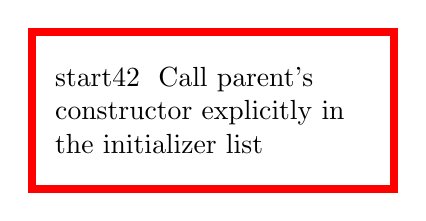
\begin{tikzpicture}
  \node[draw=red,text width=4cm,minimum height=2cm,minimum width=2cm, line width=0.1cm, inner sep=0.3cm,anchor=north east] (a) at (2,-2) 
       {\tikzmark{start42} \normalsize{ Call parent's constructor explicitly in the initializer list}};
\end{tikzpicture}
}
\begin{console}[commandchars=\~\@\$]
#include <iostream>

class P
{
public:
        P() : x_(1) { std::cout << "P::P()\n"; }
        ~textbf@P(int x) : x_(x) { std::cout << "P::P(int)\n"; }$
        int get_x() const { return x_; }
        void set_x(int x) { x_ = x; }
private:
        int x_;
};

class C: public P
{
public:
        C() : ~EMPHASIZE@P(42)$~tikzmark@end42$, x_(3), y_(2)
                     { std::cout << "C::C()"; }
        int get_y() const { return y_; }
        void set_y(int y) { y_ = y; }
private:
        int x_;
        int y_;
};

int main()
{   
    C c;
    std::cout << "c.x_ =" << c.get_x() << ", "
              << "c.y_ =" << c.get_y() << '\n';
    std::cout << "c.x_ =" << c.P::get_x() << ", "
              << "c.y_ =" << c.C::get_y() << '\n';
    return 0;
}
\end{console}
\DrawArrow[red, thick]{start42}{end42}

\begin{ex} You are given this incomplete code. Add to the
constructor of \verb!Car! and \verb!Motorcycle! so that a \verb!Car!
object is initialized to have 4 wheels and a \verb!Motorcycle! object is
initialized to have 2 wheels.
%ISSUE not sure why there are gaps in the diagram between the car and mcycle boxes, will fix in the future
\sidenote{
  \begin{tikzpicture}
  \node[draw,text width=2cm,minimum height=2cm, line width=0.05cm, inner sep=0.3cm, anchor=center] (car) at (1,-2) 
       {\tikzmark{c} \normalsize\texttt{Car}};
  \node[draw,text width=2cm,minimum height=2cm, line width=0.05cm, inner sep=0.3cm, anchor=center] (mcycle) at (4,-2) 
       {\tikzmark{m} \normalsize\texttt{Motor-\\ cycle}};
  \node[draw,text width=2cm,minimum height=2cm,minimum width=2cm, line width=0.05cm, inner sep=0.3cm, anchor=base] (vehicle) at (2.5,1) 
       {\tikzmark{v} \normalsize\texttt{Vehicle}};
  \node[above=4mm of car.north] (Lstart){};
  \node[above=4mm of mcycle.north] (Lend){};
  \node[below=6mm of vehicle.south] (Lmid){};
  \draw[ultra thick]        (car.north)   -- (Lstart) -- (Lend) -- (mcycle.north);
  \draw[ultra thick, ->]        (Lmid)   -- (vehicle.south);
\end{tikzpicture}
}
\begin{console}
class Vehicle
{
public:
        Vehicle(int numWheels)
           : numWheels_(numWheels)
        {}
        int numWheels() const { return numWheels_; }
private:
        int numWheels_;
};

class Car: public Vehicle
{
public:
        Car(bool keyless_entry)
           : keyless_entry_(keyless_entry)
        {}
private:
        bool keyless_entry_;
};

class Motorcycle: public Vehicle
{
public:
        Motorcycle()
            :
        {}
};

int main()
{   
    Car aCar;               // aCar has 4 wheels
    Motorcycle aMotorcycle; // aMotorcycle has 2
                            // wheels
    std::cout << "aCar has "
              << aCar.numWheels() << " wheels\n";
    std::cout << "aMotorcycle has "
              << aMotorcycle.numWheels()
              << " wheels\n";
    return 0;
}
\end{console}
\end{ex}
\begin{ex}
This is an incomplete piece of code:
\begin{console}
class GameObject
{
private:
        bool is_alive_;
        int x_;
        int y_;
};

class Laser: public GameObject
{
};

class Alien: public GameObject
{
};
\end{console}
\end{ex}
Add code so that during the initialization of a \verb!Laser! object, the
\verb!is_alive_! is set to \verb!false! and during the initialization
of an \verb!Alien! object, the \verb!is_alive_! is set to \verb!true!.

\newpage\EMPHASIZE{Destructor}

Now let's analyze what happens when a child object is destroyed. Of
course the child object will call it's destructor. What about the
parent's destructor?

Run the following:
\begin{console}[commandchars=\!\@\$]
#include <iostream>

class P
{
public:
        P() : x_(1) { std::cout << "P::P()\n"; }
        !textbf@~P() { std::cout << "P::~P()\n"; }$
        int get_x() const { return x_; }
        void set_x(int x) { x_ = x; }
private:
        int x_;
};

class C: public P
{
public:
        C() : x_(3), y_(2) { std::cout << "C::C()"; }
        !textbf@~C() { std::cout << "C::~C()\n"; }$
        int get_y() const { return y_; }
        void set_y(int y) { y_ = y; }
private:
        int x_;
        int y_;
};

int main()
{   
    C c;
    std::cout << "c.x_ =" << c.get_x() << ", "
              << "c.y_ =" << c.get_y() << '\n';
    std::cout << "c.x_ =" << c.P::get_x() << ", "
              << "c.y_ =" << c.C::get_y() << '\n';
return 0;
} 
\end{console}

Note that the \EMPHASIZE{child destructor} was called \EMPHASIZE{before} the
\EMPHASIZE{parent destructor}. So:
\begin{itemize}
\item
  Constructor: Parent's constructor called before child's constructor
\item
  Destructor: Child's destructor called before parent's destructor
\end{itemize}

\newpage\EMPHASIZE{Assignment operator}

If \verb!c! is a \verb!C! object and \verb!p! is a \verb!P! object, and
\verb!C! is derived from \verb!P!, can we do the following:
\begin{center}
\texttt{c = p; ???}\\
\texttt{p = c; ???}
\end{center}

\begin{console}[commandchars=\!\@\$]
#include <iostream>

class P
{
public:
        P() : x_(1) { std::cout << "P::P()\n"; }
        P(int x) : x_(x) { std::cout << "P::P(int)\n"; }
        ~P() { std::cout << "P::~P()\n"; }
        int get_x() const { return x_; }
        void set_x(int x) { x_ = x; }
private:
        int x_;
};

class C: public P
{
public:
        C() : P(42), x_(3), y_(2)
        { std::cout << "C::C()"; }
        ~C() { std::cout << "C::~C()\n"; }
        int get_y() const { return y_; }
        void set_y(int y) { y_ = y; }
private:
        int x_;
        int y_;
};

int main()
{   
    C c;
    std::cout << "c.x_ =" << c.get_x() << ", "
              << "c.y_ =" << c.get_y() << '\n';
    std::cout << "c.x_ =" << c.P::get_x() << ", "
              << "c.y_ =" << c.C::get_y() << '\n';
    P p;

    !textbf@// Which one works?$
    !textbf@c = p;$
    !textbf@p = c;$

    return 0;
} 
\end{console}
So if C is derived from \verb!P!, \verb!c! is a \verb!C! object and
\verb!p! is a \verb!P! object, then \verb!p = c;! is valid. Why?

Think about it. A \verb!C! object has more ``features'', so you can copy
those features to a \verb!P! object.

For instance suppose a child class object c has member variables c.w,
c.x, c.y, c.x and a parent class object p has member variables p.w, p.x,
then when you perform
\begin{center}
\texttt{p = c;}
\end{center}
this would happen:
\begin{center}
\texttt{p.w = c.w;}\\
\texttt{p.x = c.x;}
\end{center}
But if you attempt to do
\begin{center}
\texttt{c = p;}
\end{center}
then it's not clear what should be done for the last two assignments:
\begin{center}
\texttt{c.w = p.w;}\\
\texttt{c.x = p.x;}\\
\texttt{c.y = ????}\\
\texttt{c.z = ????}
\end{center}

\newpage\EMPHASIZE{Class Reuse: ``has-a'' and ``is-a''}

Do not confuse inheritance and composition. They re-use old classes in
different ways. Suppose \verb!P! is a class.

There are two ways to reuse \verb!P!:

\begin{itemize}
\item
  Using inheritance: \verb!C! inherits from \verb!P!
\item
  Using composition: \verb!C! contains a member that is of type \verb!P!
\end{itemize}

Look at the following example carefully. Make sure you understand what
is happening.

\sidenote{
  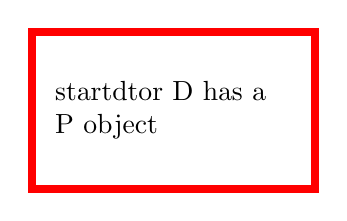
\begin{tikzpicture}
  \node[draw=red,text width=3cm,minimum height=2cm,minimum width=2cm, line width=0.1cm, inner sep=0.3cm,anchor=north east] (dtor) at (2,-2) 
       {\tikzmark{startdtor} \normalsize{D has a P object}};
\end{tikzpicture}
}
\begin{console}[commandchars=\!\@\$]
#include <iostream>

class P
{
public:
        P() : x_(1) { std::cout << "P::P()\n"; }
        P(int x) : x_(x) { std::cout << "P::P(int)\n"; }
        ~P() { std::cout << "P::~P()\n"; }
        int get_x() const { return x_; }
        void set_x(int x) { x_ = x; }
private:
        int x_;
};

class C: public P
{
public:
        C() : P(42), x_(3), y_(2)
        { std::cout << "C::C()"; }
        ~C() { std::cout << "C::~C()\n"; }
        int get_y() const { return y_; }
        void set_y(int y) { y_ = y; }
private:
        int x_;
        int y_;
};

!textbf@class D$
!textbf@{$
!textbf@public:$
        !textbf@D() : p_(42), x_(3), y_(2)$
        !textbf@{ std::cout << "D::D()"; }$
        !textbf@~D() { std::cout << "D::~D()\n"; }$
        !textbf@int get_y() const { return y_; }$
        !textbf@void set_y(int y) { y_ = y; }$
!textbf@private:$
        !textbf@P p_;$ !tikzmark@enddtor$
        !textbf@int x_;$
        !textbf@int y_;$
!textbf@};$

int main()
{   
    C c;
    std::cout << "c.x_ =" << c.get_x() << ", "
              << "c.y_ =" << c.get_y() << '\n';
    std::cout << "c.x_ =" << c.P::get_x() << ", "
              << "c.y_ =" << c.C::get_y() << '\n';
    P p;
    p = c;
    
    !textbf@D d;$

    return 0;
} 
\end{console}

\DrawArrow[red, thick]{startdtor}{enddtor}

Study the above carefully. The \verb!c! object has its own \verb!x_!
and \verb!y_! and the \verb!get_y! and \verb!set_y! methods. It also
has (through inheritance) its \verb!P::x_! and method \verb!P::get_x!
and \verb!P::set_x!. The object \verb!d! also has \verb!x_! and
\verb!y_! and the \verb!get_x! and \verb!set_x! and it also has
\verb!p_.x_! and \verb!p_.get_x! and \verb!p_.set_x!. In some
sense both \verb!c! and \verb!d! have the same ``features''.

\verb!c! has \verb!P!'s features by inheritance while \verb!d! has
\verb!P!'s features through composition.

If what you want in a class can be found in another class, should you
use composition or inheritance?

Look at ``is-a'' and ``has-a'' relationships between concepts.

Suppose you have a \verb!Vehicle! class. You want to build a \verb!Car!
class. Think about the relationship between the concept of a car and a
vehicle. Which one sounds right:

\begin{itemize}
\item
  A car ``is a'' vehicle or a vehicle ``is a'' car
\item
  A car ``has a'' vehicle or a vehicle ''has a'' car
\end{itemize}

Clearly this one sounds better.

\begin{itemize}
\item
  A car ``is a'' vehicle
\end{itemize}

This tells you that you should probably use inheritance:
\begin{console}
class Vehicle {...};
class Car: public Vehicle {...};
\end{console}

Suppose you have an \verb!Engine! class. You want to build a \verb!Car!
class. What is the relationship between an engine and a car? Which one
sounds right:

\begin{itemize}
\item
  An engine ``is a'' car or an engine ``is a'' car
\item
  An engine car ``has a'' vehicle or a vehicle ``has an'' engine
\end{itemize}

Clearly this is the best:
\begin{itemize}
\item
  A vehicle ``has an'' engine
\end{itemize}

This tells you that you should probably use composition:
\begin{console}
class Engine {...};
class Car {
...
private:
        Engine anEngine;
        ...
};
\end{console}

For composition, you want to create methods for methods in the instance
members (delegation):
\begin{console}
class Engine {
public:
        void start();
};

class Car {
public:
        void start() { anEngine.start(); }
private:
        Engine anEngine;
};
\end{console}

Users can then do this:
\begin{console}
Car honda_civic;
honda_civic.start();
// i.e., honda_civic.start() actually
// executes honda_civic.anEngine.start()
// i.e., honda_civic delegates the work of
// "start" to it' s engine
\end{console}

Otherwise you would need this:
\begin{console}
class Engine {
public:
        void start();
};

class Car {
public:
        Engine & get_engine() { return anEngine; }
private:
        Engine anEngine;
};
\end{console}

And users would have to do this:
\begin{console}
Car honda_civic;
honda_civic.get_engine().start();
\end{console}

This is \EMPHASIZE{not} so good. Why? Because you want to \EMPHASIZE{hide lower level details (engines)} and let users of your \verb!Car! class focus on higher level details (cars) which in this case is to ``start a car'' and not ``start the engine of a car''.

In terms of re-use of code:
\begin{itemize}
\item
  Derivation/inheritance is a form of white-box re-use
\item
  Composition is a form of black-box re-use
\end{itemize}

So in summary make sure you remember this:
\begin{itemize}
\item
  ``is a'' -- inheritance
\item
  ``has a'' -- composition
\end{itemize}

\begin{ex}
You want to write the Geometry Wars 2D game. You want
different shapes with different colors. To get a feel for the problem,
you want to focus on circles and squares. Circles have colors. Squares
have colors. In fact ... every shape has a color. Therefore create
a \verb!Shape! class containing color, i.e., R, G, B (\verb!int! instance variables). A circle has a radius. (HINT: Not all shapes have radius -- squares do not have radii. The location of a circle is determined by the center of the circle. A square has a width and height which are the same in value. The location of the square is determined by the coordinates of the top-left corner. A rectangle is similar to the square except that the width and height need not be the same. Write relevant classes so that if you execute this:
\begin{console}
// white circle at (2,5) of radius 3
Circle circle(2, 5, 3, 255, 255, 255);

// red square with top-left corner at (6, 7) with
// sides of length 8.
Square square(6, 7, 8, 255, 0, 0);

// green rectangle with top-left corner at (9, 10)
// with width 11 and height 12.
Rect rect(9, 10, 11, 12, 0, 255, 0);
\end{console}
\end{ex}
\newpage\EMPHASIZE{Type conversion}

Add the following to our Basic Example:
\begin{console}[commandchars=\~\@\$]
#include <iostream>

class P
{     
      ...
};

class C: public P
{
        ...
};

int main()
{   
    C c;
    ...
    P p;
    ...
    
    ~textbf@C c0(p); // This does not work!!!$
    ~textbf@P p0(c); // This works$

    return 0;
}
\end{console}

This tells you that if \verb!C! is a subclass of \verb!P!, then automatically, \verb!P! has a constructor of the form
\begin{console}
class P
{     
      ...
      P(const C &);
      ...
};
\end{console}

The default behavior of this constructor is to copy relevant values from
a \verb!C! object to the \verb!P! object that is being initialized.

This acts as a type conversion operator.

The idea is very similar to the assignment operator between objects of
\verb!C! and objects or \verb!P!. And the reason that
\begin{console}
C c0(p);
\end{console}

does NOT work is similar.

\newpage\EMPHASIZE{Multiple inheritance}

A class can be the child class of more than one parent class.

Suppose we have a \verb!Vehicle! class and a \verb!Ship! class. Then \verb!AmphibiousVehicle! is a child of both \verb!Vehicle! and \verb!Ship! class.

Syntax for multiple inheritance using public inheritance is simply:

\begin{console}
class P0 {};
class P1 {};
class C: public P0, public P1 {}; 
\end{console}

\sidenote{
  \begin{tikzpicture}
  \node[draw,text width=2cm,minimum height=2cm, line width=0.05cm, inner sep=0.3cm, anchor=center] (P0) at (1,1) 
       {\normalsize\texttt{P0}};
  \node[draw,text width=2cm,minimum height=2cm, line width=0.05cm, inner sep=0.3cm, anchor=center] (P1) at (4,1) 
       {\normalsize\texttt{P1}};
  \node[draw,text width=2cm,minimum height=2cm,minimum width=2cm, line width=0.05cm, inner sep=0.3cm, anchor=north] (C) at (2.5,-2) 
       {\normalsize\texttt{C}};
  \node[below=8mm of P0.south] (MILstart){};
  \node[below=8mm of P1.south] (MILend){};
  \node[above=11mm of C.north] (MILmid){};
  \draw[ultra thick] (MILstart) -- (MILend);
  \draw[ultra thick, ->] (MILend) -- (P1.south);
  \draw[ultra thick, <-] (P0.south) -- (MILstart);
  \draw[ultra thick] (MILmid) -- (C.north);
\end{tikzpicture}
}
Some programming languages do not allow multiple inheritance. Why?

Well, suppose class \verb!C0! is derived from \verb!P0!, \verb!P1! and both \verb!P0!, \verb!P1! have \verb!f()!. If \verb!c! is a \verb!C! object, then \verb!c.f()! is ambiguous. MAKE SURE you run the following:
\begin{console}
#include <iostream>

class P0
{
public:
        void f() {}
};

class P1
{
public:
        void f() {}
};

class C: public P0, public P1
{};

int main()
{   
    C c;
    c.f(); // which one!?!?!
    return 0;
}
\end{console}

Your C++ compiler will probably yell at you and say you have an
ambiguous invocation. This is of course the same for ambiguous member
variables:
\begin{console}
#include <iostream>

class P0
{
public:
        int x_;
};

class P1
{
public:
        int x_;
};

class C: public P0, public P1
{};

int main()
{   
    C c;
    c.x_; // which one!?!?!
    return 0;
}
\end{console}

However note that if you have two members in both parents with the same
name but you never call upon that name, your C++ will \textbf{not}
complain. For instance
\begin{console}
#include <iostream>

class P0
{
public:
        int x_;
};

class P1
{
public:
        int x_;
};

class C: public P0, public P1
{};

int main()
{   
    C c;
    return 0;
}
\end{console}

will compile. If \verb!P0! has a method that works with \verb!P0::x_! and \verb!P1! has a method that works with \verb!P1::x_!, that wouldn't be a problem:
\begin{console}
#include <iostream>

class P0
{
public:
        void f0() { std::cout << x_ << '\n'; }
        int x_;
};

class P1
{
public:
        void f1() { std::cout << x_ << '\n'; }
        int x_;
};

class C: public P0, public P1
{};

int main()
{   
    C c;
    c.f0();
    c.f1();
    return 0;
}
\end{console}

Another situation where multiple inheritance might cause a problem is
when, further up, \verb!P0! and \verb!P1! inherits from a common class:
\begin{python}
from latextool_basic import *
p = Plot()
#p += Grid(x0=-3,y0=-5,x1=3,y1=5)

G = Rect(-1, 3, 1, 5, linewidth=0.05, font=r'\huge', label=r'\texttt{G}')
P0 = Rect(-3, -1, -0.5, 1, linewidth=0.05, font=r'\huge', label=r'\texttt{P0}')
P1 = Rect(0.5, -1, 3, 1, linewidth=0.05, font=r'\huge', label=r'\texttt{P1}')
C = Rect(-1, -5, 1, -3, linewidth=0.05, font=r'\huge', label=r'\texttt{C}')

points_bottom = [(P0.bottom()), (-2, P0.bottomy()), (2, P1.bottomy()), P1.bottom(), (2, P1.bottomy()), (0, -2), (C.top())]

print(points_bottom)

p += Line(points=[(-2,-1),(-2,-2),(2,-2),(2,-1),(2,-2),(0,-2),(C.top())], linewidth=0.05)
p += Line(points=[(-2,-2),(-2,-1)], linewidth=0.05, endstyle='>')
p += Line(points=[(2,-2),(2,-1)], linewidth=0.05, endstyle='>')
p += Line(points=[(-2,1),(-2,2),(2,2),(2,1),(2,1),(2,2),(0,2),(G.bottom())], linewidth=0.05, endstyle='>')


p += G
p += P0
p += P1
p += C
print(p)
\end{python}
\begin{console}
#include <iostream>

class G
{};

class P0: public G
{};

class P1: public G
{};

class C: public P0, public P1
{};

int main()
{   
    C c;
    return 0;
}
\end{console}

The important thing to realize is that the object constructions starting
with \verb!C! is done one class at a time going up -- there are
\EMPHASIZE{two paths} in this case. The two paths don't really
``synchronize'' with each other: the creation of objects along the two
inheritance paths is independent. This means that there are \EMPHASIZE{two}
objects created with class G for \verb!c!!!!
%BIG TIKZ DIAGRAM
To verify, first do this:
\begin{console}
#include <iostream>

class G
{
public:
        int x_;
};

class P0: public G
{};

class P1: public G
{};

class C: public P0, public P1
{};

int main()
{   
    C c;
    std::cout << &(c.P0::x_) << '\n';
    std::cout << &(c.P1::x_) << '\n';
    return 0;
}
\end{console}
%THE OTHER BIG TIKZ DIAGRAM COPY
The object \verb!c! has two \verb!x_!'s. We print the address of the
two \verb!x_!'s, which of course are different:
\begin{console}
#include <iostream>

class G
{
public:
        int x_;
};

class P0: public G
{};

class P1: public G
{};

class C: public P0, public P1
{};

int main()
{   
    C c;
    std::cout << &(c.P0::x_) << '\n';
    std::cout << &(c.P1::x_) << '\n';
    return 0;
}
\end{console}

Suppose you have a game of shapes. The Shape class describes (with its
subclasses) how to draw the shape. You have another class PointMass that
computes how the shapes moves as a physical point mass. You can have:
\begin{console}
class PhysicalShape: public Shape, PointMass
{...};
\end{console}

This separates out the (motion) physics of object as a point mass from
the drawing of the object.

\begin{itemize}
\item
  If there's a draw method: it's
  probably from the \verb!Shape! class.
\item
  If there's a move method: it's
  probably from the \verb!PointMass! class
\end{itemize}

\newpage\EMPHASIZE{Public inheritance: protected member from the parent class}

Recall that our child class cannot access private members in the parent
class. (Remember that we're doing public inheritance.)

A \EMPHASIZE{protected member} (either a member variable or method) is
accessible by a subclass. Run the following:
\begin{console}[commandchars=\~\@\$]
class P
{
public: int x;
~EMPHASIZE@protected: int y_;$
private: int z_;
};

class C: public P
{
public:
void f() { y_++; } // OK
};

int main()
{   
    C c;
    ~EMPHASIZE@c.y_++;$ // WRONG!!! Will not compile!!!
    return 0;
}
\end{console}

\newpage\EMPHASIZE{Public, protected, and private}

So far you have seen public inheritance:
\begin{console}[commandchars=\~\@\$]
class P
{ ... };
class C: ~textbf@public$ P
{ ... }; 
\end{console}

There are two other types of inheritance: \EMPHASIZE{protected and private inheritance}. Suppose you have a class \verb!P!. Now define the following child classes:
\begin{console}
class CPublic: public P {};
class CProtected: protected P {};
class CPrivate: private P {}; 
\end{console}

\begin{itemize}
\item
  The private members of \verb!P! stay private in \verb!CPublic!,
  \verb!CProtected!, \verb!CPrivate!.
\item
  \verb!CPublic!: public of \verb!P! are public, protected of \verb!P!
  are protected
\item
  \verb!CProtected!: public and protected of \verb!P! are protected
\item
  \verb!CPrivate!: public, protected, and private of \verb!P! are
  private.
\end{itemize}
\begin{console}[commandchars=\~\@\$]
class P
{
~EMPHASIZE@public: int x;$
protected: int y_;
private: int z_;
};

class C: ~EMPHASIZE@public P$
{
public:
void f() { y_++; } // OK
};

int main()
{   
    C c;
    ~EMPHASIZE@c.x_++;$ // OK
    return 0;
}
\end{console}
\begin{console}[commandchars=\~\@\$]
class P
{
~EMPHASIZE@public: int x_;$
protected: int y_;
private: int z_;
};

class C: ~EMPHASIZE@protected P$
{
public:
        void f() { y_++; } // OK
};

int main()
{   
    C c;
    ~EMPHASIZE@c.x_++;$ // WRONG!!! Public x in P becomes
            // protected in C so that only subclass
            // can access x
    return 0;

}
\end{console}
\begin{console}[commandchars=\~\@\$]
class P
{
~EMPHASIZE@public: int x_;$
protected: int y_;
private: int z_;
};

class C: ~EMPHASIZE@protected P$

{

public:

void f() { y_++; } // OK

};

class C0: public C

{

public:

void f() { ~EMPHASIZE@x_++;$ } // OK. Public x becomes
                   // protected in C which
                   // is accessible in CO
};

int main()
{   
    return 0;
}
\end{console}

In summary, suppose \verb!C! is a protected subclass of \verb!P!, and \verb!x_! is a public member of \verb!P!.

\begin{itemize}
\item
  \verb!x_! is accessible in \verb!C!. (Any method in \verb!C! can
  access member \verb!x_!)
\item
  \verb!x_! becomes protected in \verb!C!. Functions outside of
  \verb!C! cannot access \verb!obj.x_! if \verb!obj! is an object of
  \verb!C!.
\end{itemize}

Note that \verb!p! is an object of \verb!P!, the \verb!p.x_! is still public.
\begin{console}[commandchars=\~\@\$]
class P
{
~EMPHASIZE@public: int x_;$
protected: int y_;
private: int z_;
};

class C: ~EMPHASIZE@private P$ // public x_ in P becomes
                   // private in C.
{
public:
        void f() { y_++; } // OK
};

class C0: public C
{
public:
        void f() { ~EMPHASIZE@x_++;$ } // WRONG!!! x_ is now private
};

int main()
{   
    return 0;
}
\end{console}

You can have as many layers of inheritance as you like:
\begin{console}
class GameObject { ... };

class Weapon: public GameObject { ... };
class Laser: public Weapon { ... };
class Rocket: public Weapon { ... };

class Spaceship: public GameObject { ... };
class AlienSoldierShip: public Spaceship { ... };
class AlienCommanderShip: public Spaceship { ... };
\end{console}

Obviously create a new class only when there are member variables and/or
methods which cannot be combined.

For instance if the following
\begin{console}
Class AlienWorth10Points {...};
class AlienWorth20Points {...};
\end{console}

have exactly the same member variables and methods except that when
objects of these types are destroyed in a gameplay, the points earned
are different, then you should have combined the two as...
\begin{console}
class Alien
{
...
    int points;
}; 
\end{console}

\newpage\EMPHASIZE{Template inheritance}

Now I want to show you how to do template inheritance. Try the following
exercise:

\begin{ex}
Write a class \texttt{\textbf{C< T >}} to be a subclass of \texttt{\textbf{P< T >}}. The class \texttt{\textbf{P< T >}} has a member variable \texttt{\textbf{x}} and method \texttt{\textbf{m()}}. The class \texttt{\textbf{C< T >}}\textbf{ }will have a member variable named \texttt{\textbf{y}} and method \texttt{\textbf{n()}}. In \texttt{\textbf{C< T >::n()}} and \texttt{\textbf{P< T >::m()}} try to access the \texttt{\textbf{x}} defined in \texttt{\textbf{P< T >}}. For simplicity make all members public.
\end{ex}
Here's the obvious first attempt at the above exercise. Run it.
\begin{console}
#include <iostream>

template < typename T >
class P
{
public:
        void m()
        {
              x = 42;
              std::cout << "P::m() ... " << x << '\n';
        }
        T x;
};

template < typename T >

class C: public P< T >
{
public:
        void n()
        {
             std::cout << "C::n() ... \n";
             x = 43;
             std::cout << x << '\n';
             std::cout << y << '\n';
        }
        T y;
};

int main()
{   
    C< int > c;
    c.n();
    c.m();
    return 0;
}
\end{console}

But there's an error! Here's the error message (if you are using g++):
\begin{console}
main.cpp: In member function 'void C< T>::n()':
main.cpp:22:9: error: ' x'{} was not declared in this
scope
22 |         x = 43;
   |         ^ 
\end{console}

Written this way, \texttt{\textbf{C< T >}} is not able to access the \texttt{\textbf{x}} member variable of \texttt{\textbf{P< T >}}. Try this:
\begin{console}[commandchars=\~\@\$]
// ... as above ...
template < typename T >
class C: public P< T >
{
public:
        void n()
        {
             std::cout << "C::n() ... \n";
             ~EMPHASIZE@this->$x = 43;
             std::cout << ~EMPHASIZE@this->$x << '\n';
             std::cout << y << '\n';
        }
        T y;
};

// ... as above ...
\end{console}
